\documentclass{article}
\usepackage[utf8]{inputenc}
\usepackage[left=1in,right=1in,top=1in,bottom=1in]{geometry}
\usepackage{crop,graphicx,array,color,flushend,stfloats,amsthm,chngpage,times,fancyhdr,lipsum,lastpage}

%%%%%%%%%%%%   Extra libraries & settings %%%%%%%%%%%%%
\setlength{\parskip}{0.25em}

%%%%%%%%%%%%   Header and Footer  %%%%%%%%%%%%%
\pagestyle{fancy}

\fancypagestyle{plain}{%
  \renewcommand{\headrulewidth}{0pt}%
  \fancyhf{}%
  \fancyfoot[R]{Page \bf\thepage\ \rm of \bf\pageref{LastPage}}%
}


%%%% Customise Titles and Headers: %%%%
\title{Don't forget adding title}
\author{Chinchuthakun Worameth (18B00033)}
\date{\today}

\fancyhf{}
\fancyhead[L]{Chinchuthakun Worameth}
\fancyhead[R]{18B00033}
\fancyfoot[R]{Page \bf\thepage\ \rm of \bf\pageref{LastPage}}


\AtBeginDocument{
%%%%%%%%%%%% Make Title and Format Lines %%%%%%%%%%%%
\maketitle											%
\vspace{-120px}										%
\noindent\rule{\linewidth}{1pt} \par				%
\vspace{100px}										%
\vspace{-20px}										%
\noindent\rule{\linewidth}{1pt} \par				%
\vspace{10px}										%
% %%%%%%%%%%%%%%%%%%% Content %%%%%%%%%%%%%%%%%%%%	
}

\AtEndDocument{
\bibliographystyle{IEEEtran}
\nocite{*}
\bibliography{citation}
}
% math stuff
\usepackage{amsmath}                % to use DeclareMathOperator
\usepackage{amssymb}
\usepackage{mathrsfs}
\usepackage{mathtools}
\usepackage{xargs}                  % for more than one optional arguments when define new commands
\usepackage{physics}                % vectors
\usepackage{mdframed}               % frames for definition, theorem, etc.
\usepackage[ruled]{algorithm2e}     % for algorithms
\usepackage{ifthen}                % for \ifthenelse
\usepackage{upgreek}

% figures and tables
\usepackage{titlesec}
\usepackage{caption}
\usepackage{subcaption}
\usepackage{multirow}
\usepackage{relsize}

% formatting some important single letters
\renewcommand{\epsilon}{\varepsilon}
\renewcommand{\phi}{\varphi}
\renewcommand{\upepsilon}{\upvarepsilon}
\renewcommand{\upphi}{\upvarphi}

% new operators
\DeclareMathOperator*{\argmin}{arg\,min}                % argmin
\DeclareMathOperator*{\argmax}{arg\,max}                % argmax
\DeclarePairedDelimiter\ceil{\lceil}{\rceil}            % ceiling function
\DeclarePairedDelimiter\floor{\lfloor}{\rfloor}         % floor function
\DeclarePairedDelimiter{\parens}{\lparen}{\rparen}      % parenthesis (use \parens* for automatically adjusting version)
\DeclarePairedDelimiter{\bracket}{[}{]}
\DeclarePairedDelimiter{\cbracket}{\{}{\}}
\DeclarePairedDelimiter{\ang}{\langle}{\rangle}
% \DeclarePairedDelimiter{\fourier}{\mathscr{F}\{}{\}}
% \DeclarePairedDelimiter{\invfourier}{\mathscr{F}^{-1}\{}{\}}

\newcommand{\fourier}[1]{\mathscr{F}\cbracket*{#1}}
\newcommand{\invfourier}[1]{\mathscr{F}^{-1}\cbracket*{#1}}
\newcommand {\dx}{\,dx}
\newcommand {\dy}{\,dy}
\newcommand {\dz}{\,dz}
\newcommand {\dt}{\,dt}
\newcommand {\du}{\,du}
\newcommand {\dtheta}{\,d\theta}
\newcommand {\domega}{\,d\omega}



\newcommand{\bigo}[1]{\ensuremath{\mathcal{O}\parens*{#1}}}
% new commands
\newcommand{\st}{such that }
\newcommand{\w}{where }
\newcommand{\del}{\nabla}
\newcommand{\larrow}{\leftarrow}
\newcommand{\rarrow}{\rightarrow}
\newcommand{\tbf}{\textbf}
\newcommand{\tit}{\textit}
\newcommand{\col}{\operatorname{col}}
\newcommand{\mat}[1]{\begin{matrix} #1 \end{matrix}}
% \newcommand{\vect}[1]{\boldsymbol{\mathbf{#1}}}
\newcommand{\vf}[1]{\boldsymbol{\mathbf{#1}}}
\newcommandx*{\seq}[2][1,2]{\ensuremath{#1, \ldots, #2}}
\newcommandx*{\ssum}[3][1,2,3]{\ensuremath{\sum_{#1 = #2}^{#3}}}
\newcommandx*{\sint}[2][1,2]{\ensuremath{\int_{#1}^{#2}}}
% \newcommandx*{\func}[4][1,2,3,4]{\ensuremath{#1^{\parens{#2}}_{#3}\parens{#4}}}
% \newcommandx*{\val}[3][1,2,3]{\ensuremath{#1^{\parens{#2}}_{#3}}}

% \newcommandx*{\func}[4][1=f,2=x,3,4, usedefault]{
%     \ifthenelse{\equal{#3}{}}{\ensuremath{#1_{#4}\parens{\vf{#2}}}}{\ensuremath{#1^{\parens{#3}}_{#4}\parens{\vf{#2}}}}
% }
\newcommandx*{\func}[3][1=f,2,3, usedefault]{
    \ifthenelse{\equal{#2}{}}{\ensuremath{#1_{#3}}}{\ensuremath{#1^{\parens{#2}}_{#3}}}
}
\newcommandx*{\val}[3][1,2,3, usedefault]{
    \ifthenelse{\equal{#2}{}}{\ensuremath{\vf{#1}_{#3}}}{\ensuremath{\vf{#1}^{\parens{#2}}_{#3}}}
}

\newcommandx*{\Real}[1][1, usedefault]{\ensuremath{\mathbb{R}^{#1}}}                % set of real number
\newcommandx*{\Int}[1][1, usedefault]{\ensuremath{\mathbb{Z}^{#1}}}                 % set of integer
\newcommandx*{\Natural}[1][1, usedefault]{\ensuremath{\mathbb{N}^{#1}}}             % set of natural number
\newcommandx*{\normal}[2][1=0, 2=1, usedefault=!]{\ensuremath{\mathcal{N}(#1,#2)}}  % Gaussian distribution

% define frame environment
% \newmdtheoremenv{definition}{Definition}
% \newmdtheoremenv{proposition}{Proposition}
% \newmdtheoremenv{corollary}{Corollary}
% \newmdtheoremenv{lemma}{Lemma}
% \newmdtheoremenv{theorem}{Theorem}
% \newmdtheoremenv{remark}{Remark}

% define keywords for algorithm
\SetKwInOut{Input}{Input}
\SetKwInOut{Output}{Output}
\SetKwInOut{Parameter}{Parameter}

% \begin{theorem}{text}{label}
% refer as \ref{tha:label}
\usepackage{tcolorbox}
\tcbuselibrary{theorems,breakable} %% を読み込む
\definecolor{burgundy}{rgb}{0.5, 0.0, 0.13}
\newtcbtheorem[number within=section]{theorem}{Theorem}%
{colframe=burgundy,colback=burgundy!2!white,
rightrule=0pt,leftrule=0pt,bottomrule=2pt,
colbacktitle=burgundy,theorem style=standard,breakable,arc=0pt}{theo}

\definecolor{oxfordblue}{rgb}{0.0, 0.13, 0.28}
\newtcbtheorem[number within=section]{definition}{Definition}%
{colframe=oxfordblue,colback=oxfordblue!2!white,
rightrule=0pt,leftrule=0pt,bottomrule=2pt,
colbacktitle=oxfordblue,theorem style=standard,breakable,arc=0pt}{def}

\definecolor{cadmiumorange}{rgb}{0.93, 0.53, 0.18}
\newtcbtheorem[number within=section]{remark}{Remark}%
{colframe=cadmiumorange,colback=cadmiumorange!2!white,
rightrule=0pt,leftrule=0pt,bottomrule=2pt,
colbacktitle=cadmiumorange,theorem style=standard,breakable,arc=0pt}{rem}

% equation numbering
\numberwithin{equation}{section}

%%%%%%%%%%%%%%%%%%%%%%%%%%%
\usepackage{listings}
\usepackage{xcolor}

\definecolor{codegreen}{rgb}{0,0.6,0}
\definecolor{codegray}{rgb}{0.5,0.5,0.5}
\definecolor{codepurple}{rgb}{0.58,0,0.82}
\definecolor{backcolour}{rgb}{0.95,0.95,0.92}

\lstdefinestyle{mystyle}{
    backgroundcolor=\color{backcolour},   
    commentstyle=\color{codegreen},
    keywordstyle=\color{magenta},
    numberstyle=\tiny\color{codegray},
    stringstyle=\color{codepurple},
    basicstyle=\ttfamily\footnotesize,
    breakatwhitespace=false,         
    breaklines=true,                 
    captionpos=b,                    
    keepspaces=true,                 
    numbers=left,                    
    numbersep=5pt,                  
    showspaces=false,                
    showstringspaces=false,
    showtabs=false,                  
    tabsize=2
}

\lstset{style=mystyle}

\makeatletter
\renewcommand*\env@matrix[1][\arraystretch]{%
  \edef\arraystretch{#1}%
  \hskip -\arraycolsep
  \let\@ifnextchar\new@ifnextchar
  \array{*\c@MaxMatrixCols c}}
\makeatother
\usepackage{subfiles}
\usepackage{subcaption}
\usepackage{hyperref}

\title{Computer Graphics Assignment \#5}
\begin{document}
\section{Question}
\begin{enumerate}
    \item Define a regular icosahedron whose center is the origin and whose one edge length is 0.8, translate the center to (0,0,-2), and make an animation that it rotates around the vertical axis which passes through the center of the icosahedron. To answer this question, use the same framework of the program and replace the plane to the icosahedron. Put one snapshot on your report and describe how to compile and execute your program.
    \item Define normal directions on vertices of the icosahedron, and apply diffuse and specular reflection effects on the surface with a point light source as if the surface of the icosahedron is like that of a sphere. The light is expected to be placed at a point that the effect of the reflections expresses efficiently. Parameters of the light and reflections are also expected to be set from the point of easy to understand the reflection effect. If you do not like a complete dark surface at backside from the light, you can adopt ambient light.
    
    The equation to calculate the intensities Rrgb is defined as
    \begin{equation}
        R_{rgb} = C_{rgb}\parens*{\max \parens*{\frac{{N\cdot{}(-L)}}{{\vert N\vert\vert L\vert}}, 0} + a}
    \end{equation}
    where $C_{rgb}$ is the color of the icosahedron, $N$ is the normal vector at a point, $L$ is the vector of an incident light direction and $a$ is a coefficient of ambient light.
\end{enumerate}

\section{Answer}
Although there are two separate questions in this assignment, this report address them together by organizing into mathematical procedure followed by implementation details for the sake of readability.

\subsection{General Procedure}
According to this discussion \cite{assignment6-ico-wikipedia}, the Cartesian coordinates of a regular icosahedron of edge length 2 centered at the origin are given by cyclic permutations of the vertices $(\pm \phi, \pm 1, 0)$ where $\phi = (1+\sqrt{5}) / 2$. Therefore, the coordinates for 12 vertices of a regular icosahedron of edge length 0.8 centered at the origin is given by
\begin{equation}
    (x,y,z) = 0.4 \times (\pm \phi, \pm 1, 0)
\end{equation}

From these coordinates, we can systematically construct 20 triangles that define the icosahedron by finding sets of three vertices such that all pairwise distance is 2. Mathematically, let $P(i)$ denotes the coordinate of $i$-th vertex, a set of all triangles $V$ is defined as
\begin{equation}
    V = \cbracket*{v = \{v_1, v_2, v_3\} ~|~ \norm{P(v_i) - P(v_j)}_2 = 2 \text{ and } v_i \in \Int_{12} ~\forall i,j \in \{1,2,3\}}
\end{equation}
where $\Int_{12} = \Int \text{ mod } 12$.

Next, given a triangle define at vertices $\val[v][][1], \val[v][][2], \val[v][][3]$, we can calculate its normal vector as
\begin{equation}
    \hat{\val[n]} = \frac{\val[p][][12] \times \val[p][][23]}{\norm{\val[p][][12] \times \val[p][][23]}_2}
\end{equation}
where $\val[p][][ij] = \val[v][][j] - \val[v][][i]$. We can check whether $\hat{\val[n]}$ is outward or inward by calculating $\val[v][][1] \cdot \hat{\val[n]}$. Specifically, the normal vector is inward is the result is greater than zero. In that case, we simply revert the direction of the normal vector and swap the order of vertices in the triangle when implementing in OpenGL. Finally, based on faces' normal vectors, we can construct normal vector at vertices by averaging normal vectors of their respective adjacent triangles.

\subsection{Implementation Details}

All vertex data, e.g. vertex coordinates, their normal vectors, and polygons they defined, are calculated in a separate \href{https://colab.research.google.com/drive/1Zi5pTD5Ymx8GxWOKJdblQa6rGU8Tv0q7?usp=sharing}{\underline{jupyter notebook}}. However, when actually implement the program using OpenGL, the source codes fail to produce the desired icosahedron for some unknown reasons. Consequently, I cannot proceed to answer the second question. I also included my incomplete implementation as well.

\begin{figure}[h]
    \centering
    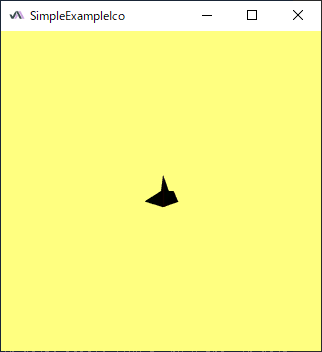
\includegraphics[width=0.4\textwidth]{figures/assignment6/cg6-snapshot.png}
    \caption{A snapshot of the animation window}
    \label{cg6-snapshot}
\end{figure}

\bibliographystyle{IEEEtran}
\bibliography{citation-assignment6}

\end{document}